\section{Aufbau}
\subsection{Apparatur 1}

  \begin{figure}[h!]
    \centering
    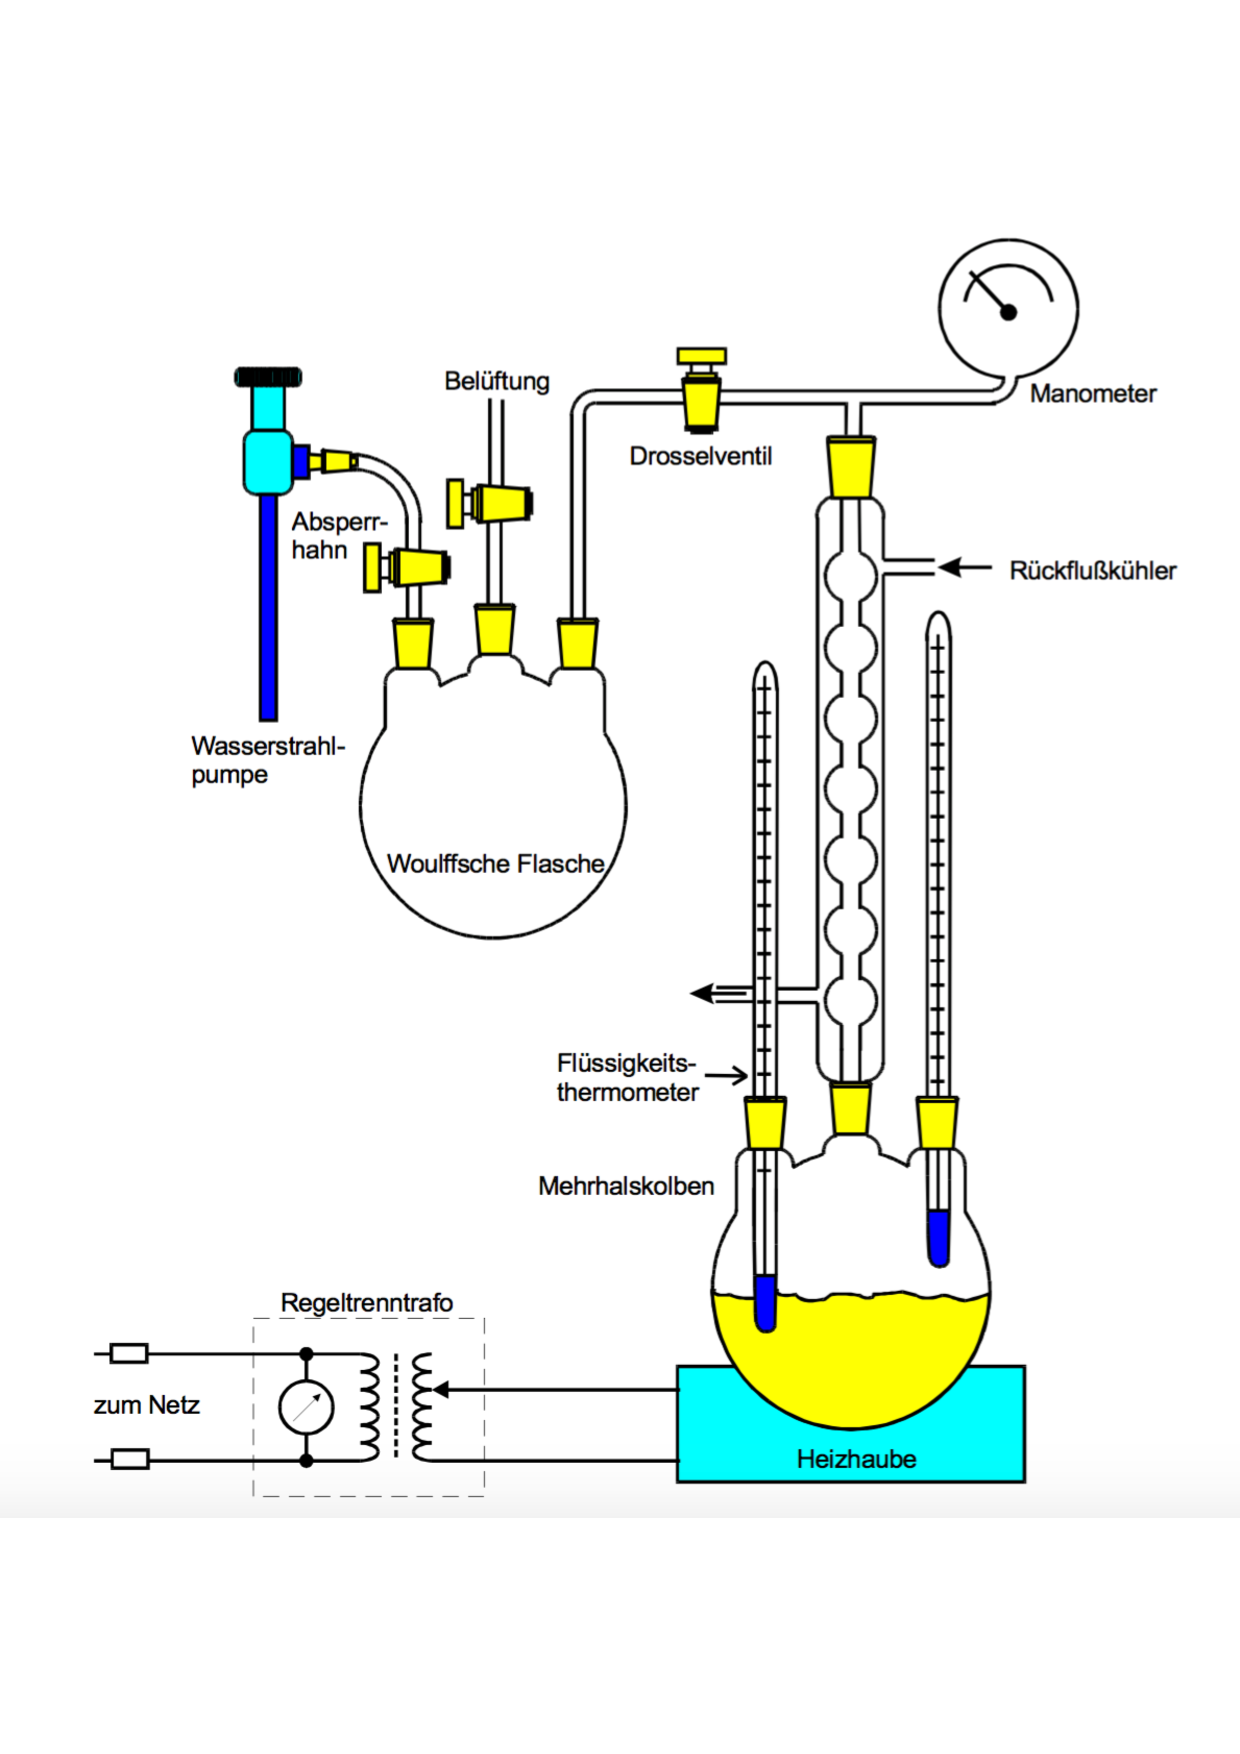
\includegraphics[height = 15cm]{Apparatur1.pdf}
    \caption{Apparatur 1 für den Druckbereich $p < 1$ \si{bar}.}
    \label{fig: Apparatur1}
  \end{figure}

\FloatBarrier

In Abbildung \ref{fig: Apparatur1} ist der Aufbau zur Bestimmung der Verdampfungswärme zu sehen.
Das Wasser wird mit Hilfe einer Heizhaube in einem evakuierten System (durch eine Wasserstrahlpumpe
realisiert) erhitzt. Die Temperatur kann
an zwei Thermometern abgelesen werden. Wobei eins in die Flüssigkeit reicht und das Andere in der
Gas-Phase misst. Der Druck wurde, anders als in der Abbildung, mit einem digitalen Messgerät gemessen.

\newpage

\subsection{Apparatur 2}

  \begin{figure}[h!]
    \centering
    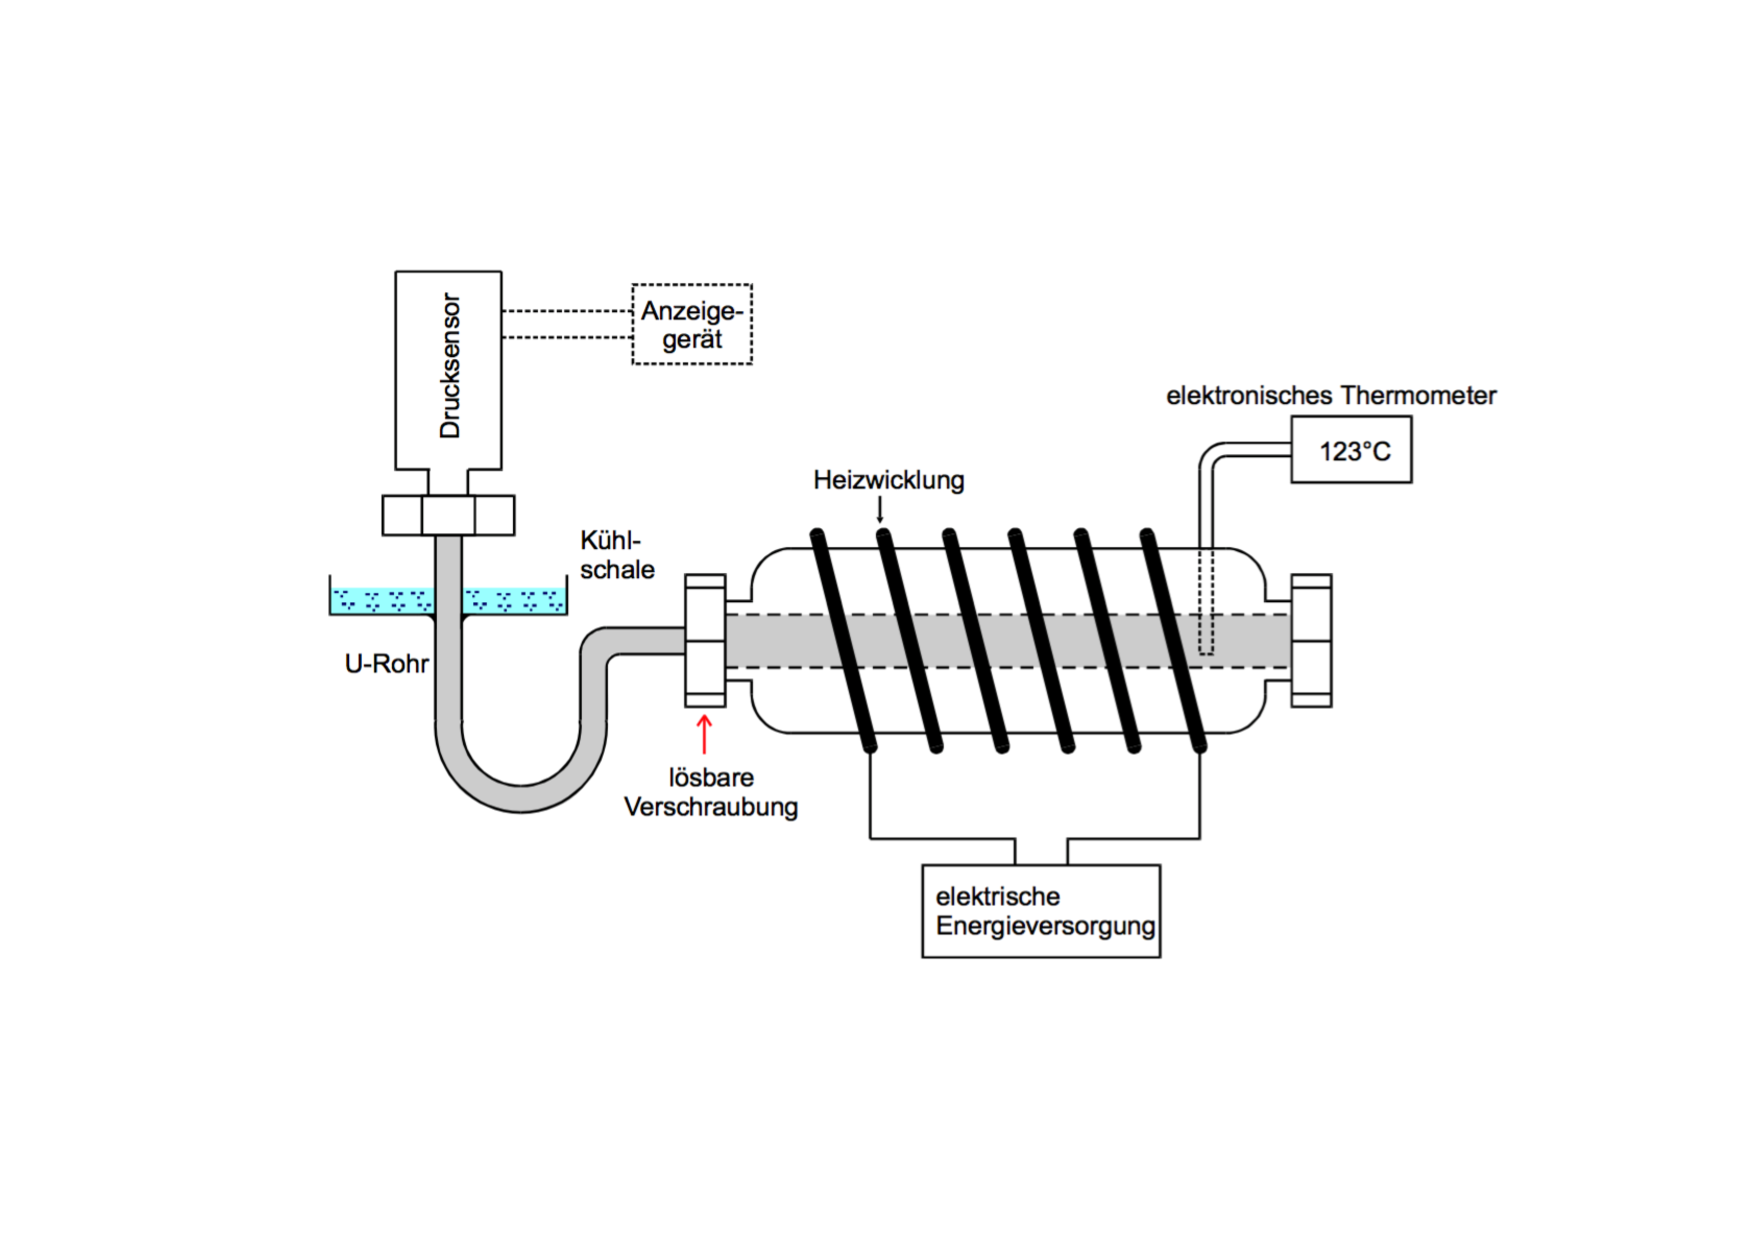
\includegraphics[height = 10cm]{Apparatur2.pdf}
    \caption{Apparatur 2 für den Druckbereich $p > 1$ \si{bar}.}
    \label{fig: Apparatur2}
  \end{figure}

\FloatBarrier

In Abbildung \ref{fig: Apparatur2} wird der Aufbau zur Messung des Drucks, in Abhängigkeit der
Temperatur, bei Werten $p > 1$ \si{bar} skizziert. Hier wurde Wasser in einem Behälter durch eine
Heizwicklung erhitzt und der Druck mit einem Drucksensor abgelesen. Ein elektronisches Thermometer
zeigt die Temperatur an.

\newpage

\section{Durchführung}
\label{sec:Durchführung}

\subsection{Apparatur 1}

Hier haben wir zunächst mit der Wasserstrahlpumpe den Druck im Innern des Sytems(so weit möglich)
gesenkt. Hierzu mussten die Ventile so geöffnet sein, dass es eine Verbindung zwischen der Pumpe
und dem Sytem gab. Nach Erreichen eines genügend kleinen Drucks wurden die Ventile geschlossen und
das Sytems so (in Bezug auf den Druck) isoliert.

Dann wurde die Heizhaube angeschaltet und zeitgleich die Durchlaufkühlung gestartet. Sobald das Wasser
siedete haben wir alle \SI{5}{\celsius} den Druck abgelesen bis zu einer Temperatur von \SI{100}{\celsius}.
Im Verlauf der Messung wurde die Kühlung immer weiter zurückgeschraubt bis sie zum Ende nur tropfenweise
lief.

\subsection{Apparatur 2}

Bei diesem Teil des Versuchs wurde zunächst der Offset bei \SI{100}{\celsius} gemessen. Dann haben wir bei
langsamem Anstieg der Temperatur alle \SI{3}{\celsius} den Druck abgelesen. Diese Messung lief bis \SI{127}{\celsius}.

\newpage
